% Options for packages loaded elsewhere
% Options for packages loaded elsewhere
\PassOptionsToPackage{unicode}{hyperref}
\PassOptionsToPackage{hyphens}{url}
\PassOptionsToPackage{dvipsnames,svgnames,x11names}{xcolor}
%
\documentclass[
  letterpaper,
  DIV=11,
  numbers=noendperiod]{scrartcl}
\usepackage{xcolor}
\usepackage[left=1in,right=1in,top=1in,bottom=1in]{geometry}
\usepackage{amsmath,amssymb}
\setcounter{secnumdepth}{-\maxdimen} % remove section numbering
\usepackage{iftex}
\ifPDFTeX
  \usepackage[T1]{fontenc}
  \usepackage[utf8]{inputenc}
  \usepackage{textcomp} % provide euro and other symbols
\else % if luatex or xetex
  \usepackage{unicode-math} % this also loads fontspec
  \defaultfontfeatures{Scale=MatchLowercase}
  \defaultfontfeatures[\rmfamily]{Ligatures=TeX,Scale=1}
\fi
\usepackage{lmodern}
\ifPDFTeX\else
  % xetex/luatex font selection
\fi
% Use upquote if available, for straight quotes in verbatim environments
\IfFileExists{upquote.sty}{\usepackage{upquote}}{}
\IfFileExists{microtype.sty}{% use microtype if available
  \usepackage[]{microtype}
  \UseMicrotypeSet[protrusion]{basicmath} % disable protrusion for tt fonts
}{}
\makeatletter
\@ifundefined{KOMAClassName}{% if non-KOMA class
  \IfFileExists{parskip.sty}{%
    \usepackage{parskip}
  }{% else
    \setlength{\parindent}{0pt}
    \setlength{\parskip}{6pt plus 2pt minus 1pt}}
}{% if KOMA class
  \KOMAoptions{parskip=half}}
\makeatother
% Make \paragraph and \subparagraph free-standing
\makeatletter
\ifx\paragraph\undefined\else
  \let\oldparagraph\paragraph
  \renewcommand{\paragraph}{
    \@ifstar
      \xxxParagraphStar
      \xxxParagraphNoStar
  }
  \newcommand{\xxxParagraphStar}[1]{\oldparagraph*{#1}\mbox{}}
  \newcommand{\xxxParagraphNoStar}[1]{\oldparagraph{#1}\mbox{}}
\fi
\ifx\subparagraph\undefined\else
  \let\oldsubparagraph\subparagraph
  \renewcommand{\subparagraph}{
    \@ifstar
      \xxxSubParagraphStar
      \xxxSubParagraphNoStar
  }
  \newcommand{\xxxSubParagraphStar}[1]{\oldsubparagraph*{#1}\mbox{}}
  \newcommand{\xxxSubParagraphNoStar}[1]{\oldsubparagraph{#1}\mbox{}}
\fi
\makeatother

\usepackage{color}
\usepackage{fancyvrb}
\newcommand{\VerbBar}{|}
\newcommand{\VERB}{\Verb[commandchars=\\\{\}]}
\DefineVerbatimEnvironment{Highlighting}{Verbatim}{commandchars=\\\{\}}
% Add ',fontsize=\small' for more characters per line
\usepackage{framed}
\definecolor{shadecolor}{RGB}{241,243,245}
\newenvironment{Shaded}{\begin{snugshade}}{\end{snugshade}}
\newcommand{\AlertTok}[1]{\textcolor[rgb]{0.68,0.00,0.00}{#1}}
\newcommand{\AnnotationTok}[1]{\textcolor[rgb]{0.37,0.37,0.37}{#1}}
\newcommand{\AttributeTok}[1]{\textcolor[rgb]{0.40,0.45,0.13}{#1}}
\newcommand{\BaseNTok}[1]{\textcolor[rgb]{0.68,0.00,0.00}{#1}}
\newcommand{\BuiltInTok}[1]{\textcolor[rgb]{0.00,0.23,0.31}{#1}}
\newcommand{\CharTok}[1]{\textcolor[rgb]{0.13,0.47,0.30}{#1}}
\newcommand{\CommentTok}[1]{\textcolor[rgb]{0.37,0.37,0.37}{#1}}
\newcommand{\CommentVarTok}[1]{\textcolor[rgb]{0.37,0.37,0.37}{\textit{#1}}}
\newcommand{\ConstantTok}[1]{\textcolor[rgb]{0.56,0.35,0.01}{#1}}
\newcommand{\ControlFlowTok}[1]{\textcolor[rgb]{0.00,0.23,0.31}{\textbf{#1}}}
\newcommand{\DataTypeTok}[1]{\textcolor[rgb]{0.68,0.00,0.00}{#1}}
\newcommand{\DecValTok}[1]{\textcolor[rgb]{0.68,0.00,0.00}{#1}}
\newcommand{\DocumentationTok}[1]{\textcolor[rgb]{0.37,0.37,0.37}{\textit{#1}}}
\newcommand{\ErrorTok}[1]{\textcolor[rgb]{0.68,0.00,0.00}{#1}}
\newcommand{\ExtensionTok}[1]{\textcolor[rgb]{0.00,0.23,0.31}{#1}}
\newcommand{\FloatTok}[1]{\textcolor[rgb]{0.68,0.00,0.00}{#1}}
\newcommand{\FunctionTok}[1]{\textcolor[rgb]{0.28,0.35,0.67}{#1}}
\newcommand{\ImportTok}[1]{\textcolor[rgb]{0.00,0.46,0.62}{#1}}
\newcommand{\InformationTok}[1]{\textcolor[rgb]{0.37,0.37,0.37}{#1}}
\newcommand{\KeywordTok}[1]{\textcolor[rgb]{0.00,0.23,0.31}{\textbf{#1}}}
\newcommand{\NormalTok}[1]{\textcolor[rgb]{0.00,0.23,0.31}{#1}}
\newcommand{\OperatorTok}[1]{\textcolor[rgb]{0.37,0.37,0.37}{#1}}
\newcommand{\OtherTok}[1]{\textcolor[rgb]{0.00,0.23,0.31}{#1}}
\newcommand{\PreprocessorTok}[1]{\textcolor[rgb]{0.68,0.00,0.00}{#1}}
\newcommand{\RegionMarkerTok}[1]{\textcolor[rgb]{0.00,0.23,0.31}{#1}}
\newcommand{\SpecialCharTok}[1]{\textcolor[rgb]{0.37,0.37,0.37}{#1}}
\newcommand{\SpecialStringTok}[1]{\textcolor[rgb]{0.13,0.47,0.30}{#1}}
\newcommand{\StringTok}[1]{\textcolor[rgb]{0.13,0.47,0.30}{#1}}
\newcommand{\VariableTok}[1]{\textcolor[rgb]{0.07,0.07,0.07}{#1}}
\newcommand{\VerbatimStringTok}[1]{\textcolor[rgb]{0.13,0.47,0.30}{#1}}
\newcommand{\WarningTok}[1]{\textcolor[rgb]{0.37,0.37,0.37}{\textit{#1}}}

\usepackage{longtable,booktabs,array}
\newcounter{none} % for unnumbered tables
\usepackage{calc} % for calculating minipage widths
% Correct order of tables after \paragraph or \subparagraph
\usepackage{etoolbox}
\makeatletter
\patchcmd\longtable{\par}{\if@noskipsec\mbox{}\fi\par}{}{}
\makeatother
% Allow footnotes in longtable head/foot
\IfFileExists{footnotehyper.sty}{\usepackage{footnotehyper}}{\usepackage{footnote}}
\makesavenoteenv{longtable}
\usepackage{graphicx}
\makeatletter
\newsavebox\pandoc@box
\newcommand*\pandocbounded[1]{% scales image to fit in text height/width
  \sbox\pandoc@box{#1}%
  \Gscale@div\@tempa{\textheight}{\dimexpr\ht\pandoc@box+\dp\pandoc@box\relax}%
  \Gscale@div\@tempb{\linewidth}{\wd\pandoc@box}%
  \ifdim\@tempb\p@<\@tempa\p@\let\@tempa\@tempb\fi% select the smaller of both
  \ifdim\@tempa\p@<\p@\scalebox{\@tempa}{\usebox\pandoc@box}%
  \else\usebox{\pandoc@box}%
  \fi%
}
% Set default figure placement to htbp
\def\fps@figure{htbp}
\makeatother





\setlength{\emergencystretch}{3em} % prevent overfull lines

\providecommand{\tightlist}{%
  \setlength{\itemsep}{0pt}\setlength{\parskip}{0pt}}



 


\usepackage{booktabs}
\usepackage{longtable}
\usepackage{array}
\usepackage{multirow}
\usepackage{wrapfig}
\usepackage{float}
\usepackage{colortbl}
\usepackage{pdflscape}
\usepackage{tabularx}
\usepackage{xltabular}
\usepackage{threeparttable}
\usepackage{threeparttablex}
\usepackage[normalem]{ulem}
\usepackage{makecell}
\usepackage{xcolor}
\usepackage{fvextra}
\DefineVerbatimEnvironment{Highlighting}{Verbatim}{breaklines,commandchars=\\\{\}}
\DefineVerbatimEnvironment{OutputCode}{Verbatim}{breaklines,commandchars=\\\{\}}
\KOMAoption{captions}{tableheading}
\makeatletter
\@ifpackageloaded{caption}{}{\usepackage{caption}}
\AtBeginDocument{%
\ifdefined\contentsname
  \renewcommand*\contentsname{Table of contents}
\else
  \newcommand\contentsname{Table of contents}
\fi
\ifdefined\listfigurename
  \renewcommand*\listfigurename{List of Figures}
\else
  \newcommand\listfigurename{List of Figures}
\fi
\ifdefined\listtablename
  \renewcommand*\listtablename{List of Tables}
\else
  \newcommand\listtablename{List of Tables}
\fi
\ifdefined\figurename
  \renewcommand*\figurename{Figure}
\else
  \newcommand\figurename{Figure}
\fi
\ifdefined\tablename
  \renewcommand*\tablename{Table}
\else
  \newcommand\tablename{Table}
\fi
}
\@ifpackageloaded{float}{}{\usepackage{float}}
\floatstyle{ruled}
\@ifundefined{c@chapter}{\newfloat{codelisting}{h}{lop}}{\newfloat{codelisting}{h}{lop}[chapter]}
\floatname{codelisting}{Listing}
\newcommand*\listoflistings{\listof{codelisting}{List of Listings}}
\makeatother
\makeatletter
\makeatother
\makeatletter
\@ifpackageloaded{caption}{}{\usepackage{caption}}
\@ifpackageloaded{subcaption}{}{\usepackage{subcaption}}
\makeatother
\usepackage{bookmark}
\IfFileExists{xurl.sty}{\usepackage{xurl}}{} % add URL line breaks if available
\urlstyle{same}
% fallback for those not using the hyperref driver hyperxmp:
\makeatletter
\@ifundefined{xmpquote}{\newcommand{\xmpquote}[1]{#1}}{}
\makeatother
\hypersetup{
  pdftitle={Investigating Voting Irregularities in the 2000 Presidential Election},
  colorlinks=true,
  linkcolor={blue},
  filecolor={Maroon},
  citecolor={Blue},
  urlcolor={Blue},
  pdfcreator={LaTeX via pandoc}}


\title{Investigating Voting Irregularities in the 2000 Presidential
Election}
\author{Marzia Rubaba and Mindy Zhang}
\date{Invalid Date}
\begin{document}
\maketitle


\subsubsection{1. Introduction}\label{introduction}

In the hard-fought U.S. Presidential election in the year 2000 between
Republican Nominee George W. Bush and Democratic nominee Al Gore, the
outcome hinged on the state of Florida. Because of a unique and
confusing butterfly ballot system in Florida's Palm Beach County, many
Democratic voters claimed their votes mistakenly went to Reform Party
candidate Pat Buchanan instead of Al Gore. Voters' confusion with the
ballot system is evident in the unusually large number of votes for
Buchanan in Palm Beach County, as well as a striking number of 19,000
ballots discarded with two circles marked. This prompts the question:
Did Buchanan receive an unusually large number of votes in Palm Beach
County than in other counties, and if so, how many of those votes may
have been intended for Gore? Using regression and prediction intervals,
this case study aims to answer this question by comparing the voting
pattern of other counties with that of Palm Beach County.

\subsubsection{2.Data Description and Exploratory Data
Analysis}\label{data-description-and-exploratory-data-analysis}

The dataset includes Bush and Buchanan's vote counts in Florida's 2000
presidential election. Palm Beach County was excluded because its
confusing butterfly ballot may have caused some Democratic voters to
accidentally vote for Buchanan. The remaining 66 counties were used to
show the usual relationship between the two candidates' votes. In these
counties, Buchanan received a median of 111 votes, while Palm Beach
County had 3,407 votes, much higher than any other county. This makes
Palm Beach County an unusual outlier.

\pandocbounded{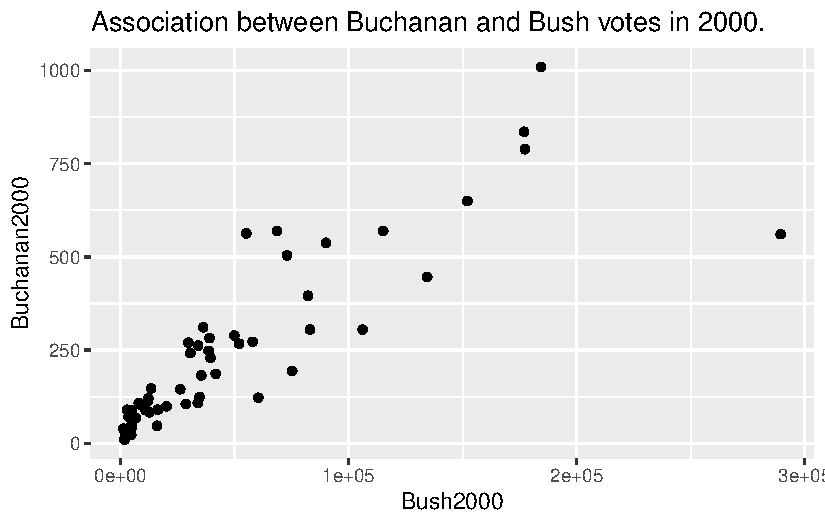
\includegraphics[keepaspectratio]{case-study-template_files/figure-pdf/unnamed-chunk-1-1.pdf}}

As shown in the scatterplot, the relationship on the original scale
displays severe right-skewness and heteroskedasticity. Most data points
cluster near the origin, and the variability in Buchanan votes widens
substantially as Bush votes increase. This fan-shaped dispersion
violates the constant variance assumption of ordinary least squares,
necessitating a natural log transformation on both variables before
fitting the regression model.

\subsubsection{3.Modeling Process}\label{modeling-process}

Let \(Buchanan_i\) denote the votes for Buchanan in 2000 in Florida
county \(i\), and \(Bush_i\) denote the votes for Bush in 2000 in
Florida county \(i\). Our final linear regression model is
\[E[log(Buchanan_i) | log(Bush_i)] = \beta_0 + \beta_1\log(Bush_i).\]

The estimated model parameters, along with their standard errors, test
statistics, and \(p\)-values, are presented in Table 1 below. The
estimated intercept is \(\hat{\beta}_0 = -2.341\)
(\(\text{SE} = 0.354\)), and the estimated slope is
\(\hat{\beta}_1 = 0.731\) (\(\text{SE} = 0.036\)). This positive slope
indicates that, holding other factors constant, every 1\% increase in
Bush votes is associated with an estimated 0.731\% increase in Buchanan
votes across the baseline counties.

\begin{table}[H]
\centering
\caption{\label{tab:unnamed-chunk-2}Table 1: Linear Regression Model for Log(Buchanan Votes) as a Function of Log(Bush Votes) (Excluding Palm Beach County)}
\centering
\begin{tabular}[t]{lcccc}
\toprule
Term & Estimate & Std. Error & t value & p-value\\
\midrule
(Intercept) & -2.341 & 0.354 & -6.61 & 9.070663e-09\\
log(Bush2000) & 0.731 & 0.036 & 20.32 & 1.300000e-29\\
\bottomrule
\end{tabular}
\end{table}

\subsubsection{4. 95\% Prediction Interval for Predicted Buchanan votes
in Palm Beach
County}\label{prediction-interval-for-predicted-buchanan-votes-in-palm-beach-county}

Assuming that the relationship between Bush votes and Buchanan votes was
the same in Palm Beach County as it was in the other counties, a 95\%
prediction interval was created using the observed votes for Bush
(152,846) in this county and the transformed fitted regression model for
the 66 other counties. The resulting interval around the fitted value of
592.3769 (Buchanan's votes) was (250.8001, 1399.164).

\subsubsection{5. Using the prediction interval to determine miscast
votes}\label{using-the-prediction-interval-to-determine-miscast-votes}

This suggests that with 152,846 votes for Bush, Palm Beach County was
predicted to display approximately 593 votes for Buchanan with a 95\%
prediction interval ranging from about 251 votes to 1400 votes. However,
the original data shows that Buchanan actually received 3,407 votes,
which significantly exceeds the upper bound of the prediction interval.
This implies that approximately 2,814 votes for Buchanan may have been
miscast in this county.

Furthermore, the prediction interval can be used to determine the range
of miscast votes by finding the difference between the observed votes
and the upper and lower bounds of the prediction interval. This gives us
a range of 2007 - 3156 for potentially miscast votes. Assuming these
excess votes were intended for Gore, our findings suggest that the
confusing butterfly ballot may have contributed to a substantial number
of voting errors in Palm Beach County.

\subsubsection{6. Limitations and
Conclusion}\label{limitations-and-conclusion}

In conclusion, our log-log regression model suggests that an unusually
large number of votes may have been mistakenly cast for Pat Buchanan in
Palm Beach County during the 2000 presidential election. The model
estimates that about 2,815 votes may have been miscast, with a 95\%
prediction interval of 2,007 to 3,156 votes. This is much larger than
George W. Bush's official 537-vote margin of victory in Florida. These
results suggest that confusion caused by the butterfly ballot may have
affected the election results.

However, our analysis has some limitations:

Generalizability limitation: Our model only uses county-level data from
Florida in the 2000 presidential election. Therefore, the results may
not apply to other states, elections, or ballot designs.

Causality and Association limitation: Our model shows a statistical
relationship, but it cannot prove that the butterfly ballot caused the
voting errors. We do not have direct evidence of what individual voters
intended to select.

Model Assumptions: Although the log-log transformation helped address
skewness and unequal variability in the data, some large-population
counties may have had a strong influence on the regression results.
Also, Palm Beach County may have differed from other counties because of
its unique population and political preferences.

\section{R Appendix}\label{r-appendix}

\begin{Shaded}
\begin{Highlighting}[]
\CommentTok{\# Loading necessary packages}
\FunctionTok{library}\NormalTok{(tidyverse)}
\FunctionTok{library}\NormalTok{(Sleuth2)}
\FunctionTok{library}\NormalTok{(broom)        }
\FunctionTok{library}\NormalTok{(kableExtra)   }

\CommentTok{\# Loading the data for case study one}
\NormalTok{election }\OtherTok{\textless{}{-}}\NormalTok{ Sleuth2}\SpecialCharTok{::}\NormalTok{ex0825}

\CommentTok{\# Creating a second dataset with Palm Beach County excluded}
\NormalTok{election\_wo\_pb }\OtherTok{\textless{}{-}}\NormalTok{ election }\SpecialCharTok{|\textgreater{}} \FunctionTok{filter}\NormalTok{(County }\SpecialCharTok{!=} \StringTok{"Palm Beach"}\NormalTok{)}

\CommentTok{\# Compute summary statistics for contextual data description}
\FunctionTok{summary}\NormalTok{(election\_wo\_pb}\SpecialCharTok{$}\NormalTok{Bush2000)}
\end{Highlighting}
\end{Shaded}

\begin{verbatim}
   Min. 1st Qu.  Median    Mean 3rd Qu.    Max. 
   1316    4745   18300   41697   54362  289456 
\end{verbatim}

\begin{Shaded}
\begin{Highlighting}[]
\FunctionTok{summary}\NormalTok{(election\_wo\_pb}\SpecialCharTok{$}\NormalTok{Buchanan2000)}
\end{Highlighting}
\end{Shaded}

\begin{verbatim}
   Min. 1st Qu.  Median    Mean 3rd Qu.    Max. 
   9.00   46.25  111.00  210.76  279.50 1010.00 
\end{verbatim}

\begin{Shaded}
\begin{Highlighting}[]
\CommentTok{\# Creating a scatterplot for the relationship between Buchanan votes and Bush votes on original scale, without Palm Beach}

\FunctionTok{ggplot}\NormalTok{(election\_wo\_pb, }\FunctionTok{aes}\NormalTok{(}\AttributeTok{x =}\NormalTok{ Bush2000, }\AttributeTok{y =}\NormalTok{ Buchanan2000)) }\SpecialCharTok{+}
  \FunctionTok{geom\_point}\NormalTok{() }\SpecialCharTok{+}
  \FunctionTok{labs}\NormalTok{(}
    \AttributeTok{title =} \StringTok{"Buchanan vs. Bush Votes (Original Scale, Excl. Palm Beach)"}\NormalTok{,}
    \AttributeTok{x =} \StringTok{"Bush Votes in 2000"}\NormalTok{,}
    \AttributeTok{y =} \StringTok{"Buchanan Votes in 2000"}
\NormalTok{  ) }\SpecialCharTok{+}
  \FunctionTok{theme\_minimal}\NormalTok{()}
\end{Highlighting}
\end{Shaded}

\pandocbounded{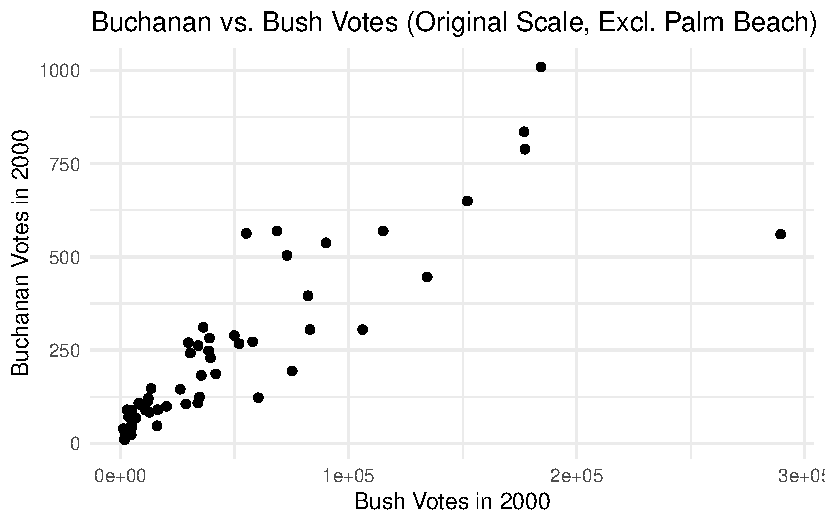
\includegraphics[keepaspectratio]{case-study-template_files/figure-pdf/unnamed-chunk-3-1.pdf}}

\begin{Shaded}
\begin{Highlighting}[]
\CommentTok{\# Scatterplot on log{-}log scale}
\FunctionTok{ggplot}\NormalTok{(election\_wo\_pb, }\FunctionTok{aes}\NormalTok{(}\AttributeTok{x =} \FunctionTok{log}\NormalTok{(Bush2000), }\AttributeTok{y =} \FunctionTok{log}\NormalTok{(Buchanan2000))) }\SpecialCharTok{+}
  \FunctionTok{geom\_point}\NormalTok{() }\SpecialCharTok{+}
  \FunctionTok{geom\_smooth}\NormalTok{(}\AttributeTok{method =} \StringTok{"lm"}\NormalTok{, }\AttributeTok{se =} \ConstantTok{FALSE}\NormalTok{, }\AttributeTok{color =} \StringTok{"steelblue"}\NormalTok{) }\SpecialCharTok{+}
  \FunctionTok{labs}\NormalTok{(}
    \AttributeTok{title =} \StringTok{"Log(Buchanan) vs. Log(Bush) Votes (Excl. Palm Beach)"}\NormalTok{,}
    \AttributeTok{x =} \StringTok{"Log(Bush Votes)"}\NormalTok{,}
    \AttributeTok{y =} \StringTok{"Log(Buchanan Votes)"}
\NormalTok{  ) }\SpecialCharTok{+}
  \FunctionTok{theme\_minimal}\NormalTok{()}
\end{Highlighting}
\end{Shaded}

\pandocbounded{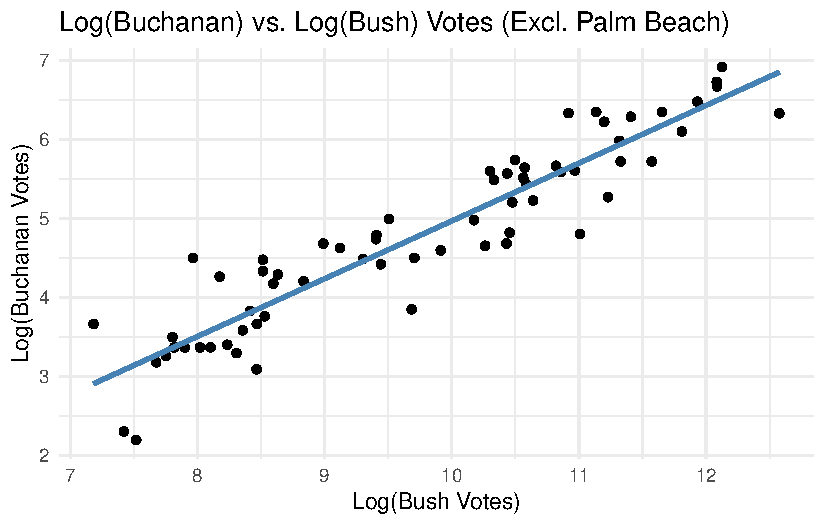
\includegraphics[keepaspectratio]{case-study-template_files/figure-pdf/unnamed-chunk-3-2.pdf}}

\begin{Shaded}
\begin{Highlighting}[]
\CommentTok{\# Creating a readable regression table for the report}
\NormalTok{election\_lm }\OtherTok{\textless{}{-}} \FunctionTok{lm}\NormalTok{(}\FunctionTok{log}\NormalTok{(Buchanan2000) }\SpecialCharTok{\textasciitilde{}} \FunctionTok{log}\NormalTok{(Bush2000), }\AttributeTok{data =}\NormalTok{ election\_wo\_pb)}
\NormalTok{election\_lm\_table }\OtherTok{\textless{}{-}} \FunctionTok{summary}\NormalTok{(election\_lm)}\SpecialCharTok{$}\NormalTok{coefficients}
\NormalTok{election\_lm\_table }\SpecialCharTok{|\textgreater{}} \FunctionTok{kbl}\NormalTok{(}\AttributeTok{col.names =} \FunctionTok{c}\NormalTok{(}\StringTok{"Term"}\NormalTok{, }\StringTok{"Estimate"}\NormalTok{, }\StringTok{"Std. Error"}\NormalTok{, }\StringTok{"t value"}\NormalTok{,}\StringTok{"p{-}value"}\NormalTok{), }\AttributeTok{align =} \StringTok{"c"}\NormalTok{, }\AttributeTok{booktabs =}\NormalTok{ T, }\AttributeTok{linesep=}\StringTok{""}\NormalTok{, }\AttributeTok{digits =} \FunctionTok{c}\NormalTok{(}\DecValTok{3}\NormalTok{, }\DecValTok{3}\NormalTok{, }\DecValTok{2}\NormalTok{, }\DecValTok{30}\NormalTok{)) }\SpecialCharTok{|\textgreater{}} \FunctionTok{kable\_classic}\NormalTok{(}\AttributeTok{full\_width =}\NormalTok{ F, }\AttributeTok{latex\_options =} \FunctionTok{c}\NormalTok{(}\StringTok{"HOLD\_position"}\NormalTok{))}
\end{Highlighting}
\end{Shaded}

\begin{table}[H]
\centering
\begin{tabular}[t]{lcccc}
\toprule
Term & Estimate & Std. Error & t value & p-value\\
\midrule
(Intercept) & -2.341 & 0.354 & -6.61 & 9.070663e-09\\
log(Bush2000) & 0.731 & 0.036 & 20.32 & 1.300000e-29\\
\bottomrule
\end{tabular}
\end{table}

\begin{Shaded}
\begin{Highlighting}[]
\CommentTok{\#. Palm Beach values }
\NormalTok{palm\_beach }\OtherTok{\textless{}{-}}\NormalTok{ election }\SpecialCharTok{|\textgreater{}} 
  \FunctionTok{filter}\NormalTok{(County }\SpecialCharTok{==} \StringTok{"Palm Beach"}\NormalTok{)}

\NormalTok{palm\_beach}
\end{Highlighting}
\end{Shaded}

\begin{verbatim}
       County Buchanan2000 Bush2000
67 Palm Beach         3407   152846
\end{verbatim}

\begin{Shaded}
\begin{Highlighting}[]
\CommentTok{\# 95\% prediction interval for Palm Beach }

\NormalTok{election\_lm\_pi }\OtherTok{\textless{}{-}} \FunctionTok{predict}\NormalTok{(}
\NormalTok{  election\_lm, }
  \AttributeTok{newdata =}\NormalTok{ palm\_beach, }
  \AttributeTok{interval =} \StringTok{"prediction"}\NormalTok{, }
  \AttributeTok{level =}\NormalTok{ .}\DecValTok{95}\NormalTok{)}
\NormalTok{pb\_pi }\OtherTok{\textless{}{-}} \FunctionTok{exp}\NormalTok{(election\_lm\_pi)}
\NormalTok{pb\_pi}
\end{Highlighting}
\end{Shaded}

\begin{verbatim}
        fit      lwr      upr
67 592.3769 250.8001 1399.164
\end{verbatim}




\end{document}
